In acest capitol vom investiga cat de mult afecteaza acestea imbunatatiri in lumea reala. Cei de la
tom's Hardware au testat procesoarele pentru a vedea daca Hyper-Threading-ul  sau functia de Tubo
Boost aduc imbunatatiri de performanta in lumea reala.


\begin{figure*}[ht] \centering
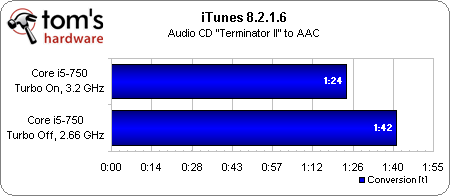
\includegraphics[width=0.6\textwidth]{img/turbo.png}
\caption{Diferenta intre Turbo Boost activat si dezactivat \cite{turbo}} \end{figure*}

Testul a fost efectuat pe softul iTunesi, un utilitar de coversie audio, deoarece acesta era un soft care folosea un singur nucleu.
Rezultatele testelor arata faptul ca desi procesorul are o frecventa de lucru mai mica decat un
single core, sau dual core, acesta este in stare sa fie la fel de rapid ca ele, in task-uri care nu
folosesc multe nuclee.

\begin{figure*}[ht] \centering
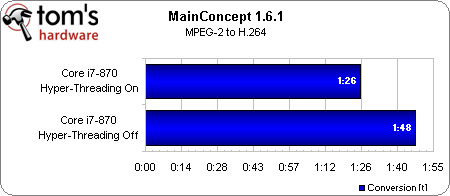
\includegraphics[width=0.6\textwidth]{img/ht1.png}
\caption{Diferenta intre cu si fara Hyper-Threading \cite{ht}} \end{figure*}


\begin{figure*}[ht] \centering
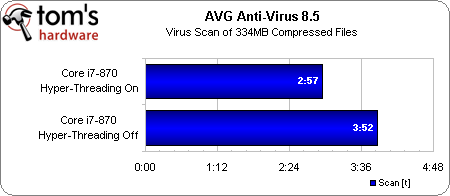
\includegraphics[width=0.6\textwidth]{img/ht2.png}
\caption{Diferenta intre cu si fara Hyper-Threading \cite{ht}} \end{figure*}

In cazul testului de hyper-threading, s-au folosit softuri optimizate pentru lucrul cu multe fire
de executie. Astfel s-a folosit MainConcept, un utilitar de conversie video si care poate folosi
mai mult de 8 nuclee, si AVG pentru scanarea fisierel, acesta find tot un program care putea rula
pe mai multe nuclee.

Din teste se observa ca desi procesorul este folosit la maxim, exista posibilitatea folosirii mai
eficienta a resurselor, astfel ca prin activarea HT, perfomanta sistemului creste.



